\chapter{The Central Theorems of Modular Arithmetic}\label{chapter:modular-arithmetic}

\section{Fermat's Little Theorem}

\begin{theorem}[Fermat's Little Theorem]\label{theorem:fermats-little-theorem}
  Consider a prime number $p$ and an integer $a$. Then the congruence
  \begin{equation*}
    a^{p}\equiv a\pmod{p}
  \end{equation*}
  holds.
\end{theorem}

\begin{proof}[Fermat's additive proof]
  Note that the congruence $(-a)^p\equiv -a^p\pmod{p}$ holds for all primes $p$, so it suffices to prove the claim for the nonnegative integers. We proceed by induction on $a$. The base case $0^p\equiv 0\pmod{p}$ clearly holds.

  For the inductive step, assume that $a^p\equiv a\pmod{p}$. The \crefnamed{theorem:binomial-theorem}{Binomial Theorem} then gives us that
  \begin{equation*}
    (a+1)^p=\sum_{k=0}^p \binom{p}{k}a^k
  \end{equation*}
  However, note that $p\mid\binom{p}{k}$ for any $0<k<p$. We therefore find that
  \begin{equation*}
    (a+1)^p\equiv a^p+1\pmod{p}.
  \end{equation*}
  Since $a^p\equiv a\pmod{p}$ holds by the induction hypothesis, the claim follows.
\end{proof}

\begin{corollary}
  Consider a prime number $p$ and an integer $a$ not divisible by $p$. Then the congruence
  \begin{equation*}
    a^{p-1}\equiv 1\pmod{p}
  \end{equation*}
  holds.
\end{corollary}

\begin{proof}
  Since $a$ is not divisible by $p$, it follows that $a$ is relatively prime to $p$, and therefore the claim follows from the cancellation law
  \begin{equation*}
    ax\equiv ay\pmod{p}\qquad\Rightarrow\qquad x\equiv y\pmod{p}.\qedhere
  \end{equation*}
\end{proof}

\begin{theorem}\label{theorem:prime-divisors-fermat-numbers}
  If $p$ is a prime divisor of a Fermat number $F_n:=2^{2^n}+1$, then
  \begin{equation*}
    p\equiv 1\pmod{2^{n+1}}
  \end{equation*}
\end{theorem}

\begin{corollary}
  The fourth Fermat number $2^{2^4}+1=65537$ is prime.
\end{corollary}

\begin{proof}
  Any prime divisor of $F_4=2^{2^4}+1$ must satisfy the congruence $p\equiv 1\pmod{33}$. If $F_4$ is composite, then it must have a prime divisor below $\sqrt{F_4}$, and thus below $2^8=256$. The sieve of Eratosthenes displayed in \cref{figure:sieve-of-eratosthenes} reveals that the only two primes $p\equiv 1\pmod{33}$ below $256$ are $97$ and $193$. A quick computation gives that
  \begin{equation*}
    F_4\equiv 62\pmod{97}\qquad\text{and}\qquad F_4\equiv 110\pmod{193},
  \end{equation*}
  so that neither $97$ nor $193$ is a prime divisor of $F_4$, and therefore we conclude that $F_4$ is prime.
\end{proof}

\begin{corollary}
  The fifth Fermat number $2^{2^5}+1=4,294,967,297$ is composite with prime factor
  \begin{equation*}
    641\mid 2^{2^5}+1.
  \end{equation*}
\end{corollary}

It is widely believed, and strongly supported by evidence, that every Fermat number is square-free.

\section{Euler's Theorem}

Euler figured out a way to generalize Fermat's Little Theorem to the composite moduli. He made use of his totient function $\phi$, which counts for each $n$ the number of $0\leq m<n$ relatively prime to $n$.

\begin{theorem}[Euler's Theorem]\label{theorem:eulers-theorem}
  Consider a natural number $n$ and an integer $a$ such that $\gcd(a,n)=1$. The congruence
  \begin{equation*}
    a^{\phi(n)}\equiv 1\pmod{n}
  \end{equation*}
  holds
\end{theorem}

We present two proofs of Euler's Theorem. The first is the standard proof, and the other is inspired by methods of group theory.

\begin{proof}[First proof of Euler's Theorem]
  Consider an integer $a$ relatively prime to $n$, and consider a reduced residue system $r_1,\ldots,r_{\phi(n)}$ modulo $n$. We claim that
  \begin{equation*}
    ar_1,\ldots,ar_{\phi(n)}
  \end{equation*}
  is again a reduced residue system modulo $n$. Indeed, since multiplying by $a$ induces a bijection on $\mathbb{Z}/n\mathbb{Z}$, we see that all integers $ar_1,\ldots,ar_{\phi(n)}$ are incongruent. Furthermore, the product of any two integers relatively prime to $n$ is again relatively prime to $n$, so all the integers $ar_i$ are relatively prime to $n$. Since any set of $\phi(n)$ incongruent integers relatively prime to $n$ form a reduced residue system, the claim follows.

  Using that the integers $ar_1,\ldots,ar_{\phi(n)}$ form a reduced residue system, it follows that
  \begin{equation*}
    \prod_{i=1}^{\phi(n)}r_i\equiv \prod_{i=1}^{\phi(n)}ar_i = a^{\phi(n)}\prod_{i=1}^{\phi(n)}r_i\pmod{n}
  \end{equation*}
  Since $\prod_{i=1}^{\phi(n)}r_i$ is relatively prime to $n$, it follows that $a^{\phi(n)}\equiv 1\pmod{n}$.
\end{proof}

\begin{proof}[Second proof of Euler's Theorem]
  Consider the least positive integer $k$ such that $a^k\equiv 1\pmod{n}$, and consider the relation $\sim$ on the set of integers $0\leq b<n$ relatively prime to $n$, where
  \begin{equation*}
    b\sim c \qquad\text{if and only if}\qquad \exists_{0\leq i< k} ba^i\equiv c\pmod{n}.
  \end{equation*}
  This relation is reflexive, because $ba^0 \equiv b\pmod{n}$. It is symmetric, because if $ba^i\equiv c\pmod{n}$ for some nonzero $i$, then $ca^{k-i}\equiv ba^ia^{k-i}\equiv b\pmod{n}$. Furthermore, it is transitive, because if $ba^i\equiv c$ and $ca^j\equiv d$, then $ba^{i+j}\equiv d$. If $k\leq i+j$, then we find that also $ba^{i+j-k}\equiv d$. Thus, the relation $\sim$ is an equivalence relation.

  We claim that each equivalence class has size $k$. Indeed, for each $b$, the set
  \begin{equation*}
    \{b,ba,ba^2,\ldots,ba^{k-1}\}
  \end{equation*}
  consists of $k$ distinct elements, because multiplying with $b$ is a bijection. Thus we have partitioned the set of all numbers $0\leq b<n$ relatively prime to $n$ into equivalence classes of size $k$. On the other hand, the total number of elements $0\leq b<n$ relatively prime to $n$ is the number $\phi(n)$. This shows that $k\mid \phi(n)$, so it follows that $a^{\phi(n)}\equiv 1\pmod{n}$.
\end{proof}

\begin{remark}
  The second proof of Euler's theorem can be simplified using the language of group theory. A \emph{group} is a set $G$ equipped with a binary operation $x,y\mapsto xy$, a unary operation $x\mapsto x^{-1}$, and a unit element $1$, satisfying the axioms
  \begin{align*}
    (xy)z & = x(yz) \\
    x1 & = x \\
    1x & = x \\
    xx^{-1} & = 1 \\
    x^{-1}x & = 1.
  \end{align*}
  One can show that the set of integers modulo $n$ relatively prime to $n$ forms a group, where the binary operation is multiplication, the unit element is the integer $1$, and the inverse $x^{-1}$ of an integer $x$ modulo $n$ is the unique solution to the equation $xy\equiv 1\pmod{n}$. The number of elements in this group is $\phi(n)$. For any integer $a$ modulo $n$ relatively prime to $n$ such that $a^k\equiv 1\pmod{n}$, the set $\{1,a,a^2,\ldots,a^{k-1}\}$ is a subgroup, which means that it is closed under the group operations. The argument where we introduced an equivalence relation $\sim$ to partition the set of all integers modulo $n$ relatively prime to $n$ into equivalence classes of size $k$ is an instance of a much more general result, Lagrange's Theorem, which asserts that the size of any subgroup of a finite group divides the size of the entire group.
\end{remark}

Since $\phi(p)=p-1$, it follows that \crefnamed{theorem:fermats-little-theorem}{Fermat's Little Theorem} is also a direct corollary of \crefnamed{theorem:eulers-theorem}{Euler's Theorem}.

Some questions about Euler's totient function remain unresolved. While we have seen that $\phi(p)=p-1$ for any prime number $p$, Lehmer asked whether there is any composite number $n$ such that
\begin{equation*}
  \phi(n)\mid n-1.
\end{equation*}
This open problem is now known as \emph{Lehmer's problem} \cite{lehmer1933}.

\section{Wilson's Theorem}

The following theorem was first published by Edward Waring, who attributed it as follows to John Wilson \cite[p.~380]{waring1782} along with high praise: \textit{This most elegant property of prime numbers was discovered by the most illustrious and most skilled mathematician, John Wilson, Esquire.} However, neither Wilson nor Waring were able to rigorously prove this property of the prime numbers. The first to give a proof was Joseph--Louis Lagrange \cite{lagrange1771}. Euler, and later Gauss, gave separate proofs of this fact.

\begin{theorem}[Wilson's Theorem]\label{theorem:wilsons-theorem}
  A natural number $n$ is prime if and only if
  \begin{equation*}
    (n-1)!\equiv -1 \pmod{n}.
  \end{equation*}
\end{theorem}

\begin{proof}
  First, we observe that the claim holds for $n=2$, since $1\equiv -1\pmod{2}$.
  
  Suppose that $n$ is prime strictly greater than $2$. Then every integer $0<a<n$ has a multiplicative inverse modulo $n$, i.e., for every integer $a$ there is an integer $a^{-1}$ such that
  \begin{equation*}
    aa^{-1}\equiv 1.
  \end{equation*}
  Now we group the integers $1\leq a < n$ into pairs with their own inverses.
  By \cref{exercise:self-inverse-modulo-prime} and the assumption that $n\neq 2$, there are exactly two integers that would pair up with themselves because they are their own inverses: The integers $1$ and $-1$ are the only two integers $a$ modulo $n$ for which the congruence $a^2\equiv 1\pmod{n}$ holds. The other integers come in proper pairs $(a,a^{-1})$.

  Each pair $(a,a^{-1})$ contributes $1$ to the product
  \begin{equation*}
    (n-1)!:=\prod_{a=1}^{n-1}a.
  \end{equation*}
  Therefore, there is exactly one factor that contributes a something to this product: the factor $-1$. Thus we see that $(n-1)!\equiv -1\pmod{n}$.

  Conversely, suppose that the congruence $(n-1)!\equiv -1\pmod{n}$ holds. Then it follows that
  \begin{equation*}
    -(n-1)!\equiv 1\pmod{n}.
  \end{equation*}
  For any proper divisor $a$ of $n$, we therefore find that $a$ divides $1$ modulo $n$, i.e., that there is a solution to the linear congruence
  \begin{equation*}
    ax\equiv 1\pmod{n}.
  \end{equation*}
  This implies that $\gcd(a,n)=1$. It follows that the only proper divisor of $n$ is $1$, i.e., that $n$ is prime.
\end{proof}

\section{Lucas's Theorem}

\crefnamed{theorem:kummers-theorem}{Kummer's Theorem} gave a complete characterization of the prime factorization of binomial coefficients. In principle, this is sufficient to know the congruence class of $\binom{n}{m}$ modulo a prime $p$. In the following theorem, which is due to \'Edouard Lucas, we establish a pattern.

\begin{theorem}
  Consider a prime number $p$, and natural numbers $m$ and $n$ written in base $p$ as
  \begin{equation*}
    m=\sum_{i=0}^ka_ip^i\qquad\text{and}\qquad n=\sum_{i=0}^kb_ip^i.
  \end{equation*}
  Then the congruence
  \begin{equation*}
    \binom{n}{m}\equiv\prod_{i=0}^k\binom{b_i}{a_i}\pmod{p}
  \end{equation*}
  holds.
\end{theorem}

\section{The Quadratic Character of \texorpdfstring{$-1$}{-1}}

\begin{wrapfigure}[19]{r}{0.4\textwidth}
  \centering
  \begin{tikzpicture}
    \node[inner sep=0pt, rounded corners=0.2em, clip] {%
      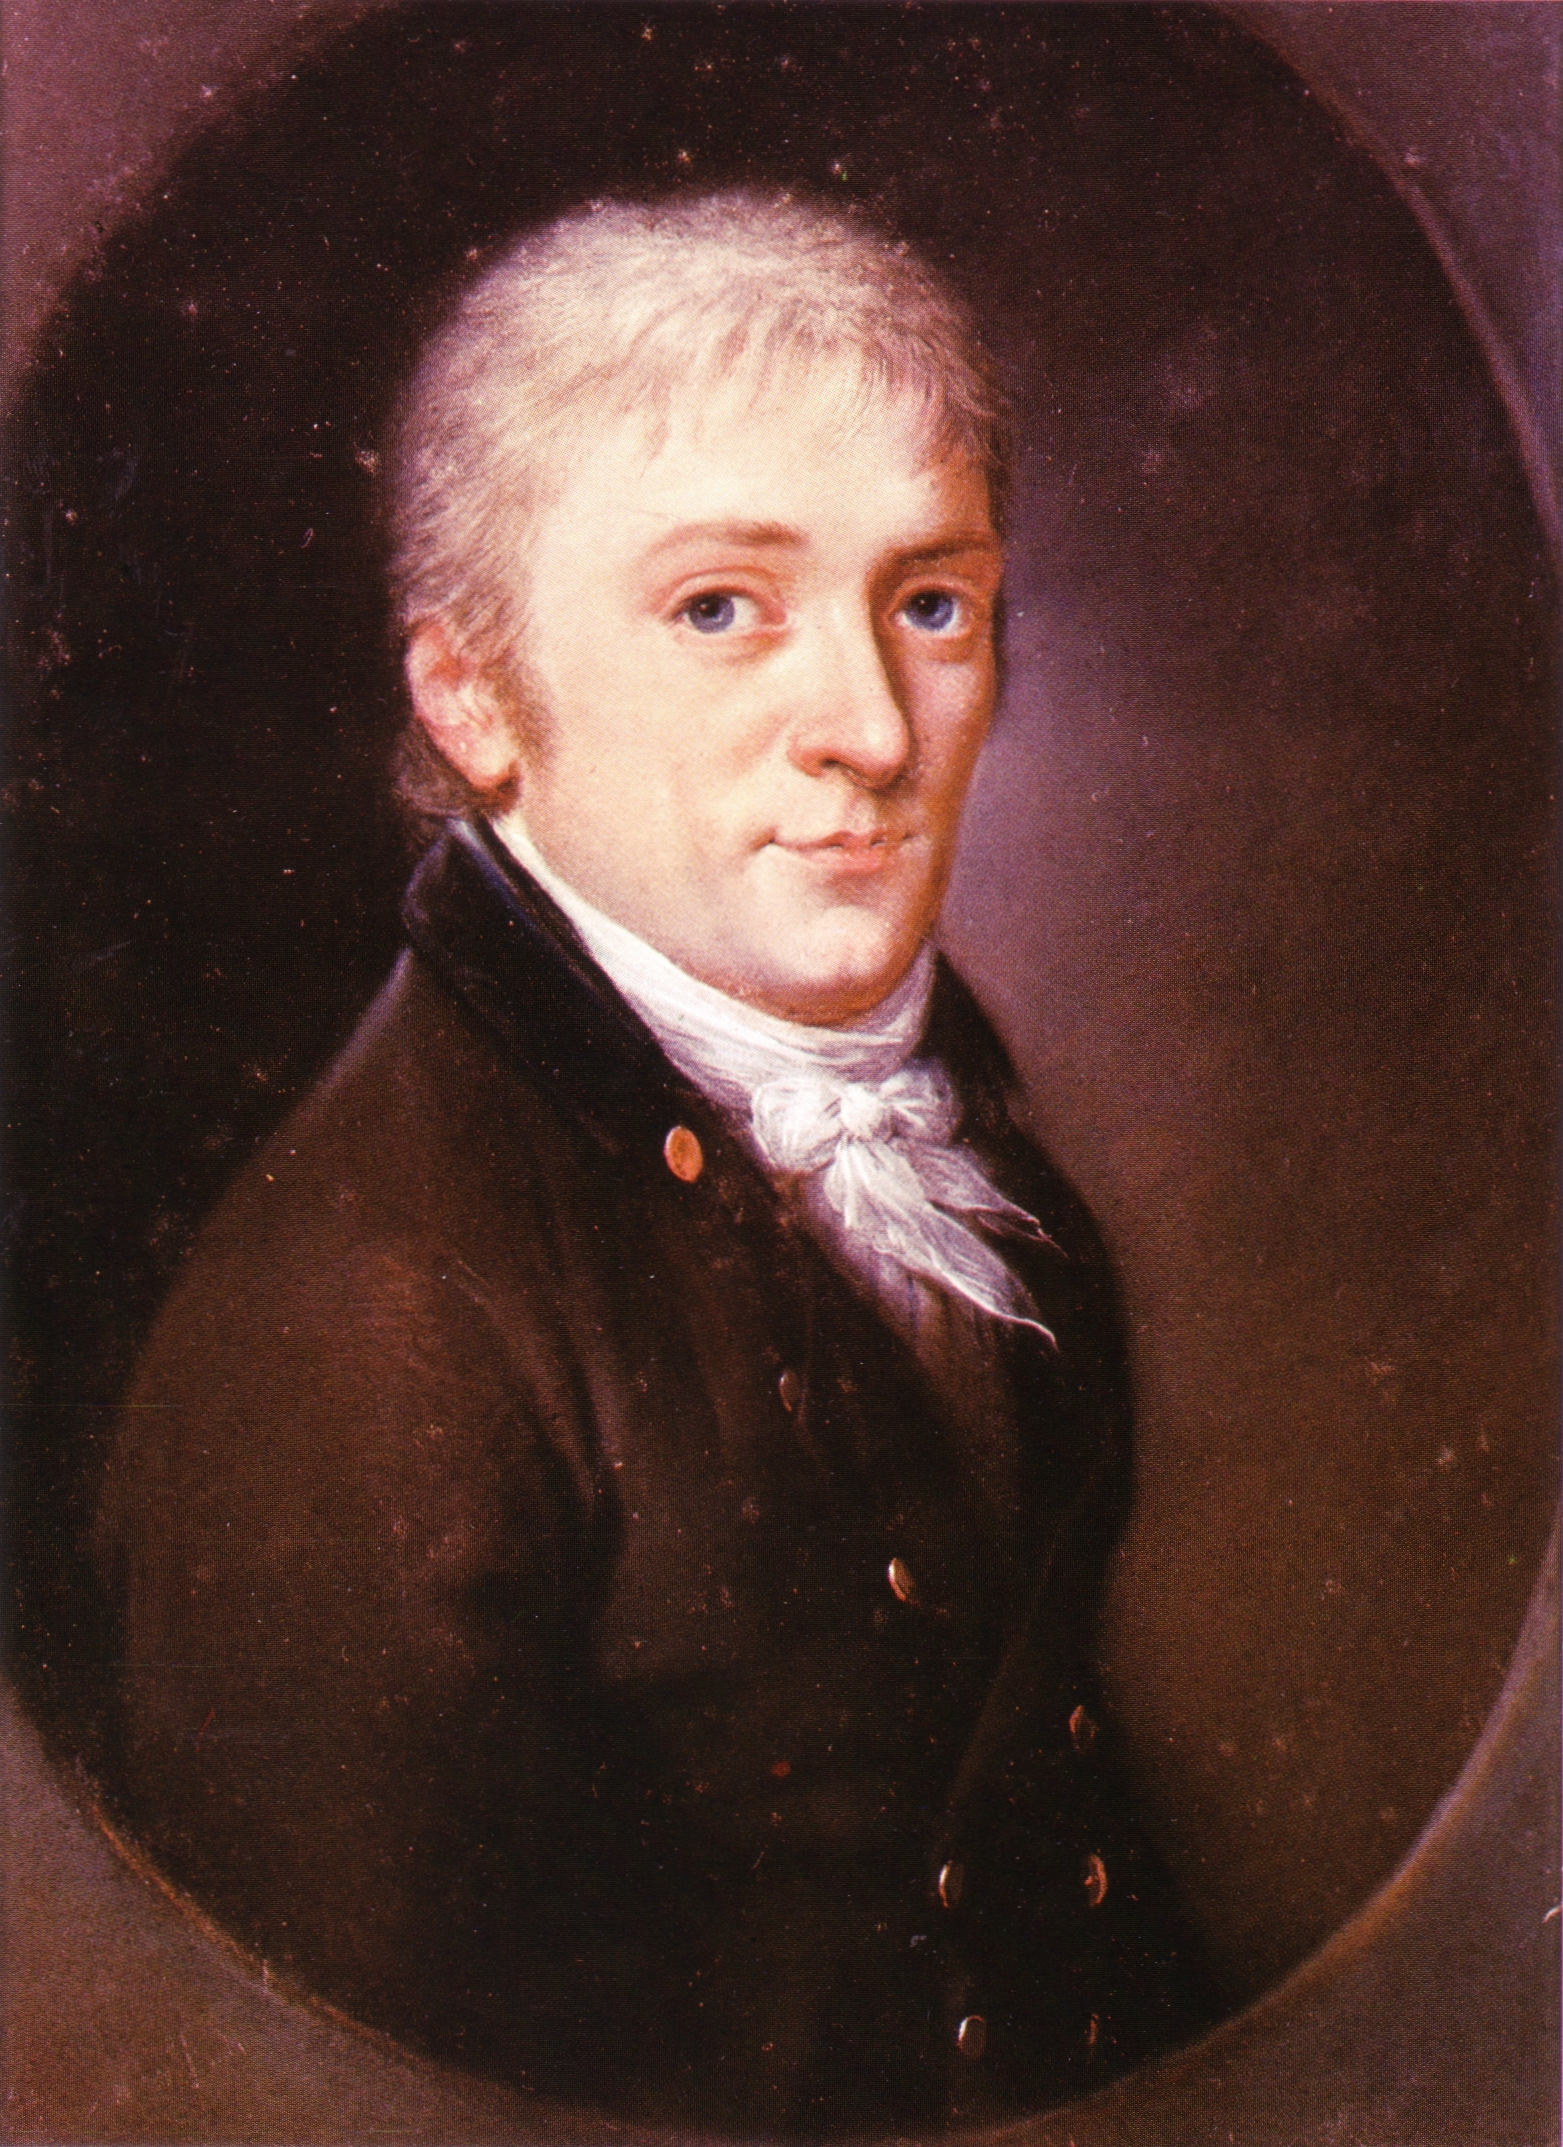
\includegraphics[width=0.32\textwidth]{gauss1803.jpg}%
    };
  \end{tikzpicture}
  \caption[Carl Friedrich Gauss]{\sloppy{Carl Friedrich Gauss. Pastel painting by Johann Christian August Schwartz, 1803.}}
  \label{fig:gauss}
\end{wrapfigure}
\crefnamed{theorem:wilsons-theorem}{Wilson's Theorem} can be used to prove a historically important result in the development of modular arithmetic: that $-1$ is congruent to a square modulo an odd prime $p$ if and only if $p\equiv 1\pmod{4}$.
In his \emph{Disquisitiones Arithmeticae} \cite{gauss1986}, Gauss writes of this result that when he encountered it in 1795---he was 19 at the time---he considered it to be a result of rare beauty and suspected deep connections with even
more profound results, that he concentrated all his efforts into understanding its underlying principles. He became so attracted by the questions of this nature, that he could not let them be. Ultimately, Gauss's investigations into higher arithmetic, as he preferred to call it, led him to prove the celebrated \crefnamed{theorem:quadratic-reciprocity}{Law of Quadratic Reciprocity}.

While the law of quadratic reciprocity is certainly the central theorem of our subject, the quadratic character of $-1$ modulo a prime is a key result on its own. In this section we will show that it can be used to show that there are infinitely many primes congruent to $1$ modulo $4$. Furthermore, we will use the fact that $-1$ is congruent to a square modulo $p$ when $p\equiv 1\pmod{4}$ in the next chapter to prove Fermat's \emph{Two-Square Theorem}, which asserts that every such prime is the sum of two squares. Questions similar to the quadratic character of $-1$ modulo a prime will be investigated more fully in \cref{chapter:quadratic-residues,chapter:quadratic-reciprocity}.

\begin{theorem}\label{theorem:quadratic-character-neg-1}
  Consider an odd prime $p$. Then there exists an integer $a$ such that
  \begin{equation*}
    a^2\equiv-1\pmod{p}
  \end{equation*}
  if and only if $p\equiv 1\pmod{4}$.
\end{theorem}

\begin{proof}
  First, we show that if there is an integer $a$ such that $a^2\equiv-1\pmod{p}$, then we must have $p\equiv 1\pmod{4}$. By \crefnamed{theorem:fermats-little-theorem}{Fermat's Little Theorem} it follows that
  \begin{equation*}
    (-1)^{\frac{p-1}{2}}\equiv (a^2)^{\frac{p-1}{2}} \equiv a^{p-1}\equiv 1\pmod{p}
  \end{equation*}
  This shows that $\frac{p-1}{2}$ must be even, which is equivalent to the congruence $p\equiv 1\pmod{4}$.
  
  For the converse, assume that $p\equiv 1\pmod{4}$. By \crefnamed{theorem:wilsons-theorem}{Wilson's Theorem} we know that $(p-1)!\equiv -1\pmod{p}$. Now, observe that the integers $1,\ldots,p-1$ can be arranged in pairs, where each $i$ is paired with $p-i$, which is always distinct from $i$ because $p-1$ is even. Since $i(p-i)\equiv -i^2\pmod{p}$, we obtain the congruences
  \begin{equation*}
    -1\equiv(p-1)!\equiv (-1)^{\frac{p-1}{2}}\left(\left(\frac{p-1}{2}\right)!\right)^2\equiv\left(\left(\frac{p-1}{2}\right)!\right)^2\pmod{p}.
  \end{equation*}
  The last congruence holds, because $(p-1)/2$ is even by the assumption that $p\equiv 1\pmod{4}$. Thus, we have presented $-1$ as a square modulo $p$.
\end{proof}

The previous theorem describing the quadratic character of $-1$ modulo an odd prime $p$ can be used to show that there are infinitely many primes congruent to $1$ modulo $4$. The first fifteen primes congruent to $1$ modulo $4$ are:
\begin{equation*}
  5,~13,~17,~29,~37,~41,~53,~61,~73,~89,~97,~101,~109,~113,~\text{and}~137.
\end{equation*}

\begin{theorem}
  There are infinitely many primes congruent to $1$ modulo $4$.
\end{theorem}

\begin{proof}
  Consider a finite set of primes $p_1,\ldots,p_k$ that are all congruent to $1$ modulo $4$, and define
  \begin{equation*}
    n = (2p_1\cdots p_k)^2 + 1.
  \end{equation*}
  Notice that $n\equiv 1\pmod{4}$ is greater than $1$, and $p_i\nmid n$ for any $1\leq i\leq k$. It follows that for any prime divisor $q$ of $n$, we have
  \begin{equation*}
    (2p_1\cdots p_k)^2\equiv -1\pmod{q},
  \end{equation*}
  showing that $-1$ is a quadratic residue modulo $q$. Since $-1$ is a quadratic residue modulo $q$ if and only if $q\equiv 1\pmod{4}$, it follows that any prime divisor $q$ of $n$ is congruent to $1$ modulo $4$. Since none of the prime divisors of $n$ are among the primes $p_i$ we started out with, the primes $p_i$ could not have listed all the primes congruent to $1$ modulo $4$.
\end{proof}

\section{The Infinitude of Primes Congruent to 1 Modulo Powers of 2}

One way to show that a prime $p$ is congruent to $1$ modulo $n$ is by finding an integer $a$ such that
\begin{equation*}
  \ord_p(a)=n.
\end{equation*}
By the \crefnamed{theorem:order-theorem}{Order Theorem} and \crefnamed{theorem:fermats-little-theorem}{Fermat's Little Theorem}, this implies that $n\mid p-1$. We will use this idea to show that there are infinitely many primes congruent to $1$ modulo any power of $2$. In particular, there are infinitely many primes congruent to $1$ modulo $4$, modulo $8$, modulo $16$, and so on.

\begin{theorem}\label{theorem:infinitude-of-primes-1-mod-power-of-2}
  For any positive natural number $n$, there are infinitely many primes congruent to $1$ modulo $2^n$.
\end{theorem}

\begin{proof}
  Since $p\equiv 1\pmod{2^{n+1}}$ implies that $p\equiv 1\pmod{2^n}$, it suffices to show that for any finite list $p_1,\ldots,p_k$ of primes congruent to $1$ modulo $2^{n+1}$, there is a prime $q\equiv 1\pmod{2^{n+1}}$ which is not among the primes $p_i$.

  Given such a list of primes $p_i$, let
  \begin{equation*}
    a:=2p_1\cdots p_k,
  \end{equation*}
  and let $q$ be a prime divisor of the integer $b:=a^{2^n}+1$. Note that $q$ is necessarily an odd prime, since $a$ is even and hence $b$ is odd. Since $p_i\nmid b$ for any $i$, it follows that $q$ is not among the primes $p_i$. Furthermore, we observe that
  \begin{equation*}
    a^{2^n}\equiv -1\pmod{q}.
  \end{equation*}
  This implies that $\ord_q(a)\mid 2^{n+1}$, while clearly $\ord_q(a)\nmid 2^n$. Thus, we must have $\ord_q(a)=2^{n+1}$, and this allows us to conclude that $q\equiv 1\pmod{2^{n+1}}$.
\end{proof}

The previous theorem is a special case of a deep theorem in analytic number theory: \emph{Dirichlet's Theorem}. Dirichlet's Theorem shows that for any integer $a$ relatively prime to $n$, there are infinitely many primes
\begin{equation*}
  p\equiv a\pmod{n}.
\end{equation*}
The techniques of proving Dirichlet's Theorem are beyond the scope of this course. However, having taken this course, you are well equipped to read LeVeque's excellent \emph{Topics in Number Theory} \cite{leveque1956vol1,leveque1956vol2}, a two-volume work that contains well-explained proofs of Dirichlet's Theorem as well as the Prime Number Theorem.

\begin{exercises}
  \exercise For every prime $p\equiv 1\pmod{4}$ below $100$, find the least positive integer $a$ such that $a^2\equiv -1\pmod{p}$.
  \exercise Consider an odd prime $p=2n+1$. Show that
  \begin{equation*}
    \binom{2n}{n}\equiv (-1)^{\frac{p-1}{2}}\pmod{p}.
  \end{equation*}
  \exercise
  \begin{subexenum}
  \item Consider a prime $p$ and an integer $p\nmid a$. Show that
    \begin{equation*}
      a^p\equiv a\pmod{p^2}\qquad\Leftrightarrow \qquad a^{p^2}\equiv a\pmod{p^2}.
    \end{equation*}
  \item A prime satisfying $a^p\equiv a\pmod{p^2}$ is called a \emph{Wieferich prime base $a$}. Wieferich encountered this condition by showing that if $x^p+y^p=z^p$ with $p\nmid xyz$, then $p$ must be a Wieferich prime base $2$ \cite{wieferich1909}. The only known Wieferich primes base $2$ are $p=1093$ and $p=3511$, and there are no smaller Wieferich primes base $2$.
    
    In bases larger than $2$ there are smaller Wieferich primes, although they are still rare. The only known Wieferich primes base $3$ are $p=11$ and $p=1006003$. Show that $5$ is a Wieferich prime base $32$.
  \end{subexenum}
  \exercise For any positive integer $n$ we define the \emph{Euler quotient}
  \begin{equation*}
    q_n(x):=\frac{x^{\phi(n)}-1}{n},
  \end{equation*}
  where $x$ is assumed to be relatively prime to $n$. In the special case where $n$ is a prime, $q_n(x)$ is called the \emph{Fermat quotient}. Show that
  \begin{equation*}
    q_n(ab)\equiv q_n(a)+q_n(b)\pmod{n}
  \end{equation*}
  for any two integers $a$ and $b$ relatively prime to $n$.
  \exercise Consider two integers $a$ and $b$, and a prime number $p$. Show that
  \begin{equation*}
    (a+b)^p\equiv a^p+b^p\pmod{p}.
  \end{equation*}
  \exercise Show that
  \begin{equation*}
    2^{p-2}+3^{p-2}+6^{p-2} \equiv 1 \pmod{p}
  \end{equation*}
  for any prime number $p\neq 3$.
  \exercise
  \begin{subexenum}
  \item Prove that
    \begin{equation*}
      5^{5^5}\equiv 5^5\pmod{31}.
    \end{equation*}
  \item Prove that
    \begin{equation*}
      7^{7^7}\equiv 7^7\pmod{43}.
    \end{equation*}
  \item Find a prime $p>3$ such that
    \begin{equation*}
      3^{3^3}\equiv 3^3\pmod{p}.
    \end{equation*}
  \end{subexenum}
  \exercise Show that
  \begin{equation*}
    3^{3^{3^3}}\equiv 3^{3^3}\pmod{97}.
  \end{equation*}
  \exercise Consider two primes $p$ and $q$. Show that
  \begin{equation*}
    pq\mid (13^p-5^p)(13^q-5^q)\qquad\Leftrightarrow\qquad pq\mid 12.
  \end{equation*}
  \exercise
  \begin{subexenum}
  \item Show that any number of the form
    \begin{equation*}
      m^5n-n^5m
    \end{equation*}
    is divisible by $30$.
  \item Show that for any two odd primes $p$ and $q$, the number
    \begin{equation*}
      p^5q-q^5p
    \end{equation*}
    is divisible by $240$.
  \end{subexenum}
  \exercise Prove that if
  \begin{equation*}
    a^n\equiv a \pmod{n}
  \end{equation*}
  for every integer $a$, then $n=2$ or $n$ is odd.
  \exercise Find all the solutions to the equation
  \begin{equation*}
    p^q-q^p=p+q,
  \end{equation*}
  where $p$ and $q$ are prime numbers.
  \exercise For any integer $a$ and any prime number $p$, show that
  \begin{equation*}
    a^{p^k} \equiv a^{p^{k-1}} \pmod{p^k}.
  \end{equation*}
  \exercise Consider two distinct primes $p$ and $q$, and an integer $a\geq 0$. Prove that
  \begin{equation*}
    a^{pq}+a\equiv a^p + a^q \pmod{pq}
  \end{equation*}
  \exercise
  \begin{subexenum}
  \item Show that the number $6481=3^8-3^4+1$ is prime. Hint: In order to avoid trying out all the primes below $80$, show first that every prime factor $p$ of $6481$ satisfies $p\equiv 1\pmod{24}$.
  \item Compute the prime factorization of the number
    \begin{equation*}
      3^{24}-1.
    \end{equation*}
  \end{subexenum}
  \exercise Show that the congruence
  \begin{equation*}
    \sum_{k=1}^{n} k^n\equiv 0\pmod{n}
  \end{equation*}
  holds if and only if $n$ is odd.
  \exercise. Find the least integer $k>1$ such that every integer of the form $x^k-x$ is divisible by $47$ and $89$.
\end{exercises}

%%% Local Variables:
%%% mode: latex
%%% TeX-master: "elementary-number-theory"
%%% End:
